\subsubsection{Sections}

\textbf{Section} identifies code \textbf{sections to be divided among all threads}.

\highspace
Sections allow to specify that the enclosed section(s) of code are to be executed in parallel. \textbf{Each section is executed once by a thread in the team}.

\marginpar{
    \href{https://www.openmp.org/spec-html/5.0/openmpsu37.html\#x59-1010002.8.1} {Doc. \faIcon{book}}
}
\begin{openmpbox}[: sections]
\begin{lstlisting}[language=C++]
#pragma omp [parallel] sections [clauses]
{
    #pragma omp section
    {
        code_block
    }
}\end{lstlisting}
\end{openmpbox}

\noindent
The sections directive identifies a noniterative work-sharing construct that specifies a set of constructs that are to be divided among threads in a team. Each section is executed once by a thread in the team.

\highspace
Each section is preceded by a \texttt{section} directive, although the \texttt{section} directive is optional for the first section. The \texttt{section} directives must appear within the lexical extent of the \texttt{sections} directive. There's an \textbf{implicit barrier} at the end of a \texttt{sections} construct, unless a \texttt{nowait} is specified.

\highspace
Restrictions to the sections directive are as follows:
\begin{itemize}
    \item A \texttt{section} directive must not appear outside the lexical extent of the \texttt{sections} directive.
    \item Only a single \texttt{nowait} clause can appear on a \texttt{sections} directive.
\end{itemize}

\begin{figure}[!htp]
    \centering
    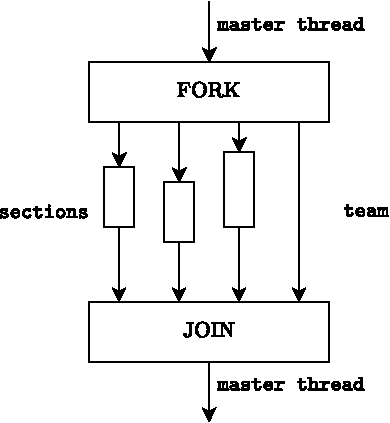
\includegraphics[width=.45\textwidth]{img/openmp-sections-1.pdf}
    \caption{Breaks work into separate, discrete sections, each executed by a thread (functional parallelism).}
\end{figure}
